% !TeX root = ../thesis.tex

\chapter{Introduction}
\label{sec:introduction}
Within the last few years, substantial research in deep learning networks for object detection have enabled the autonomous vehicles to develop rapidly and achieve promising performance. Rather than simply detecting the road the vehicle is driving on, the surrounding people and vehicles, how they act and how to respond are also crucial in determining the possible future trajectories and realizing the safe driving. The ability to sense the surrounding environment is called perception, including multiple subdomains such as objection detection\cite{girshick_rich_2014}, classification\cite{krizhevsky_imagenet_2017}, simultaneous localization and mapping (\acrshort{slam})\cite{smith_estimating_2013,montemerlo_fastslam_nodate}. Astounding advances in computer vision have been achieved in the last decade and undoubtedly its ability can rival or even surpass human in many areas. Before the emergence of deep learning, a time-consuming method “the sliding window”\cite{enzweiler_monocular_2009} is used to detect objects, in which a rectangle window moves over the image to find the target object and the classifier has to be applied in each window to classify the interested image. Methods relying on neutral network and the advance in reliable perception systems facilitate the tasks of object detection to be more efficient and accurate. The invention of \acrshort{cnn}\cite{lecun_backpropagation_1989} made the milestone contribution to deep learning algorithms and the application in computer vision, such as \acrshort{rcnn}\cite{girshick_rich_2014},Fast R-CNN\cite{girshick_fast_2015}, \acrshort{yolo}\cite{redmon_you_2016}, consecutively improvement in which achieving a progressively performance in object detection work.

Considering onboard sensors used to assess the surroundings, cameras have been well accepted for many years due to the price advantage and relatively clear recognition. However, 2D image is not qualified to provide deeply scene perception required in automotive and industrial robotics, while the astonishing development in 3D sensors, such as ToF (time-of-flight), \acrshort{lidar}, stereo vision etc., light up the future of object detection. \acrshort{lidar}, short for Light Detection and Ranging, is equipped in many autonomous vehicles to capture 3D scene information with the representation of sparse and irregular point clouds. Comparing with the conventional camera, \acrshort{lidar} sensor is capable of providing high-resolution \(360^{\circ}\) 3D information, as shown in Figure \(\ref{fig:lidar scan range}\), by discretizing the vertical space in line with hundreds of points.  In the object detection work, the raw point clouds generated by \acrshort{lidar} sensor will go through a preprocess firstly, and then be fed into a detection model, the output of which will be post-processed to make predictions. The advantages of \acrshort{lidar}, such as accurate estimation of object sizes when many similar colored objects exist and less affected by bad lighting via providing own infrared light source, make it considerably competitive in autonomous driving, especially under adverse weather conditions.

\begin{figure}[!htbp]
\centering
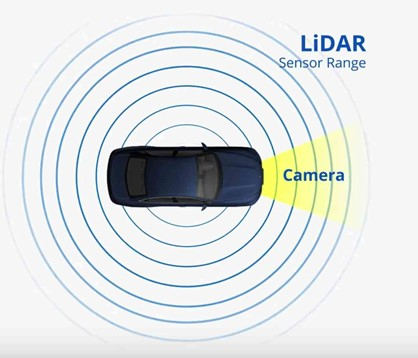
\includegraphics[scale=0.6]{Graphics/Lidar scan range.jpg}
\caption{The horizontal scan range of \acrshort{lidar} and camera\cite{Lidar}}
\label{fig:lidar scan range}
\end{figure}

The high reliability of the point cloud information makes \acrshort{lidar}-based perception become more and more welcomed and adopted in autonomous vehicles industry, but inevitably \acrshort{lidar} has its limitation, for instance, the difficulty of detection exponentially increases with the distance from the object. Moreover, recent studies point out that occlusion patterns in \acrshort{lidar} point clouds can be ignored and severely threaten the credibility of detection\cite{sun_towards_nodate}.  Specifically, when one vehicle is driving behind another one, the point cloud displays fewer points because the front vehicle occludes the \acrshort{lidar} beams. Inability to learn occlusion information makes \acrshort{lidar} point clouds expose to spoofing attacks, which encourage further exploration in the underlying misclassification of object detection imperatively.

Many studies have shown that small perturbations in the input sample, which are even imperceptible to human vision, can prompt the model to make a substantially incorrect prediction with high confidence\cite{papernot_limitations_2015,szegedy_intriguing_2014},\cite{goodfellow_explaining_2015} possibly leading to devastating consequences in the real world such as car crashes and fatal injuries\cite{kurakin_adversarial_2017,Uber}. This vulnerability of neural network restricts its application in security-critical area and make model robustness test under different scenarios increasingly needed. “Adversarial examples” was firstly introduced by Szegedy et al.\cite{szegedy_intriguing_2014} in the image classification work,  generating the perturbed examples by exploring the minimal necessary perturbations to maximize the prediction error, and adversarial examples have transferability property which can be used to attack on diverse models\cite{szegedy_intriguing_2014,goodfellow_explaining_2015,liu_delving_2017,papernot_transferability_2016,naseer_cross-domain_2019}. After the revelation of the existence of adversarial examples,  multitude researchers dedicate to inspecting how robust a neural network can be and how to strengthen networks against the attacks\cite{huang_learning_2016,gu_towards_2015,bastani_measuring_2017,shaham_understanding_2018}, activating a fresh study domain “adversarial attack and defense”.  

Concerning the categories of threat model, adversarial attacks can be classified into white box, grey box and black box, depending on the degree of knowledge acquired by the adversary. White-box attack assumes the adversary has comprehensive knowledge of the target model, therefore, crafting adversarial samples on the target model is relatively simple and direct, and most well-known attack algorithms are designed based on white-box model. The knowledge of the adversary in the grey-box attacks is limited, with only the information of target model structure\cite{ferrari_gray-box_2018}. In the black-box attacks, the attacker has no access to the target model parameters\cite{sun_towards_nodate,liu_delving_2017,papernot_practical_2017}.  Innovative and progressive attack algorithms come out continuously during the last couple of years, such as \acrshort{fgsm}\cite{goodfellow_explaining_2015}, \acrshort{pgd}\cite{kurakin_adversarial_2017}, \acrshort{cw}\cite{carlini_towards_2017}, \acrshort{jsma}\cite{papernot_limitations_2015}, DeepFool\cite{moosavi-dezfooli_deepfool_2016}. 

To increase the network robustness against above enumerated attacks, defense approaches are urgently required, which generally includes adversarial training\cite{szegedy_intriguing_2014}, denoising methods\cite{zhou_dup-net_2019,xie_feature_2019,xu_feature_2018}, randomization-based schemes\cite{luo_random_2020,athalye_synthesizing_2018}, provable defenses\cite{raghunathan_certified_2020}, and detection of adversarial examples before feeding into the networks\cite{meng_magnet_2017,liu_detection_2018}. Amid the current defense mechanisms, none of them can manifest both efficient and effective against existing adversarial samples, all bearing either deficiency of computational intractability or fragility to adaptive white-box attacks to some extent. Conceivable explanations accounting for the obstacles in constructing defense mechanisms are as following: lack of powerful theoretical tools to solve complicated optimization problems which are commonly used to generate adversarial samples,  impracticable of deep learning to produce good outputs for each possible input. Defenses techniques with high adaptivity and effectiveness 

Adversarial attacks for 2D image data is well explored in recent research as introduced above\cite{szegedy_intriguing_2014,goodfellow_explaining_2015,moosavi-dezfooli_deepfool_2016,papernot_limitations_2015,carlini_towards_2017}, but studies on the vulnerability of point cloud network is not sufficient until now. Extending 2D adversarial attacks approaches to point clouds is a challenging task, considering the following reasons: 

1. Raw point clouds are situated in coordinates \(xyz\), without pixel information that can be modified. 

2. The positions of points are arbitrary which enlarge the search space for adversarial samples. 

3. \(L_{p}\) norm that is widely accepted in 2D adversarial attack is not applicable in point clouds data regarding to the properties of irregularity and varying cardinality\cite{xiang_generating_2019}. So far, 3D adversarial attack approach is composed of following categories: gradient-based method such as FGSM\cite{goodfellow_explaining_2015} and its variants\cite{gu_towards_2015,kurakin_adversarial_2017,dong_boosting_2018,madry_towards_2019,liu_extending_2019}, optimization-based method represented by C\&W\cite{carlini_towards_2017} and L-BFGS\cite{szegedy_intriguing_2014}, skeleton-detach based approach\cite{yang_adversarial_2019} and GAN-based method\cite{zhou_lg-gan_nodate,vedaldi_advpc_2020}. 

Heretofore, most attack approaches are proved to be theoretically feasible under preset scenarios and carefully-crafted adversarial sample datasets. Considering the potential applications in security-critical systems such as autonomous vehicles and the unpredictable nature of 3D data which can be affected by lighting or noise in adverse weather, comprehensive understanding of robustness on practical examples in the real world is of paramount importance. To the best of our knowledge, physically attacks on 3D point clouds are simulated in some recent works, for instance, setting obstacles under different distance and orientation\cite{cao_adversarial_2019}, placing adversarial objects on the rooftop of a vehicle\cite{tu_physically_2020}, simulating "hide objects" by randomly removing original points in ground-truth bounding box\cite{hau_object_2021} These attempts prove that existing state-of-the-art detection networks are disappointingly susceptible to attacks and pose highly concern on the practical applications. In spite of the poor results, these endeavours are very meaningful to call for and shed light on more future effort in 3D point cloud detection.

In this paper, we are aiming at exploring the robustness of 3D point cloud object dection networks. The experiment is composed of four sections: In the first section, we extend FGSM algorithm and its variants, which are widely used in image domain and point cloud classification area, to 3D point cloud objetct detection, and carry out attacks and defenses on the neural network, specifically PointPillars\cite{lang_pointpillars_2019}. In the second section, we perform adversarial attacks by the means of dropping critical points, which is inspired by Zheng et al.\cite{zheng_pointcloud_2019} PointPillars use a simplified PointNet\cite{qi_pointnet_2017} to capture critical features, and we define critical points according to the abstracted critical features. Attacks in the first two sections are based on detection models, a new adversarial attack approach not relying on a specific model is introduced in the section three. We create benchmark datasets by either adding Gaussian noise or randomly drop points to test the volunerability of the models. In the last section, we augment dataset by integrating simulated point clouds of adverse weather. 

The paper is constructed as follows: The first section describes the pertinent background and motivation , formalize the problem 
In the second section, related literature about object detection and adversarial attack and defenses are briefly introduced.  Section 3 will provide detailed description of the dataset and methodology. Section 4 will present the experiment settings and results of attacks and defense and analysis. The last section summarizes the conclusion and discuss the future directions.
